\section{Methods}

We manually designed strategies that organisms could use to cooperate to experimentally demonstrate that the dishtiny framework selects for detectable hierarchical transitions of individuality.

\subsection{dishtiny}

\begin{figure*}[t]
\begin{center}
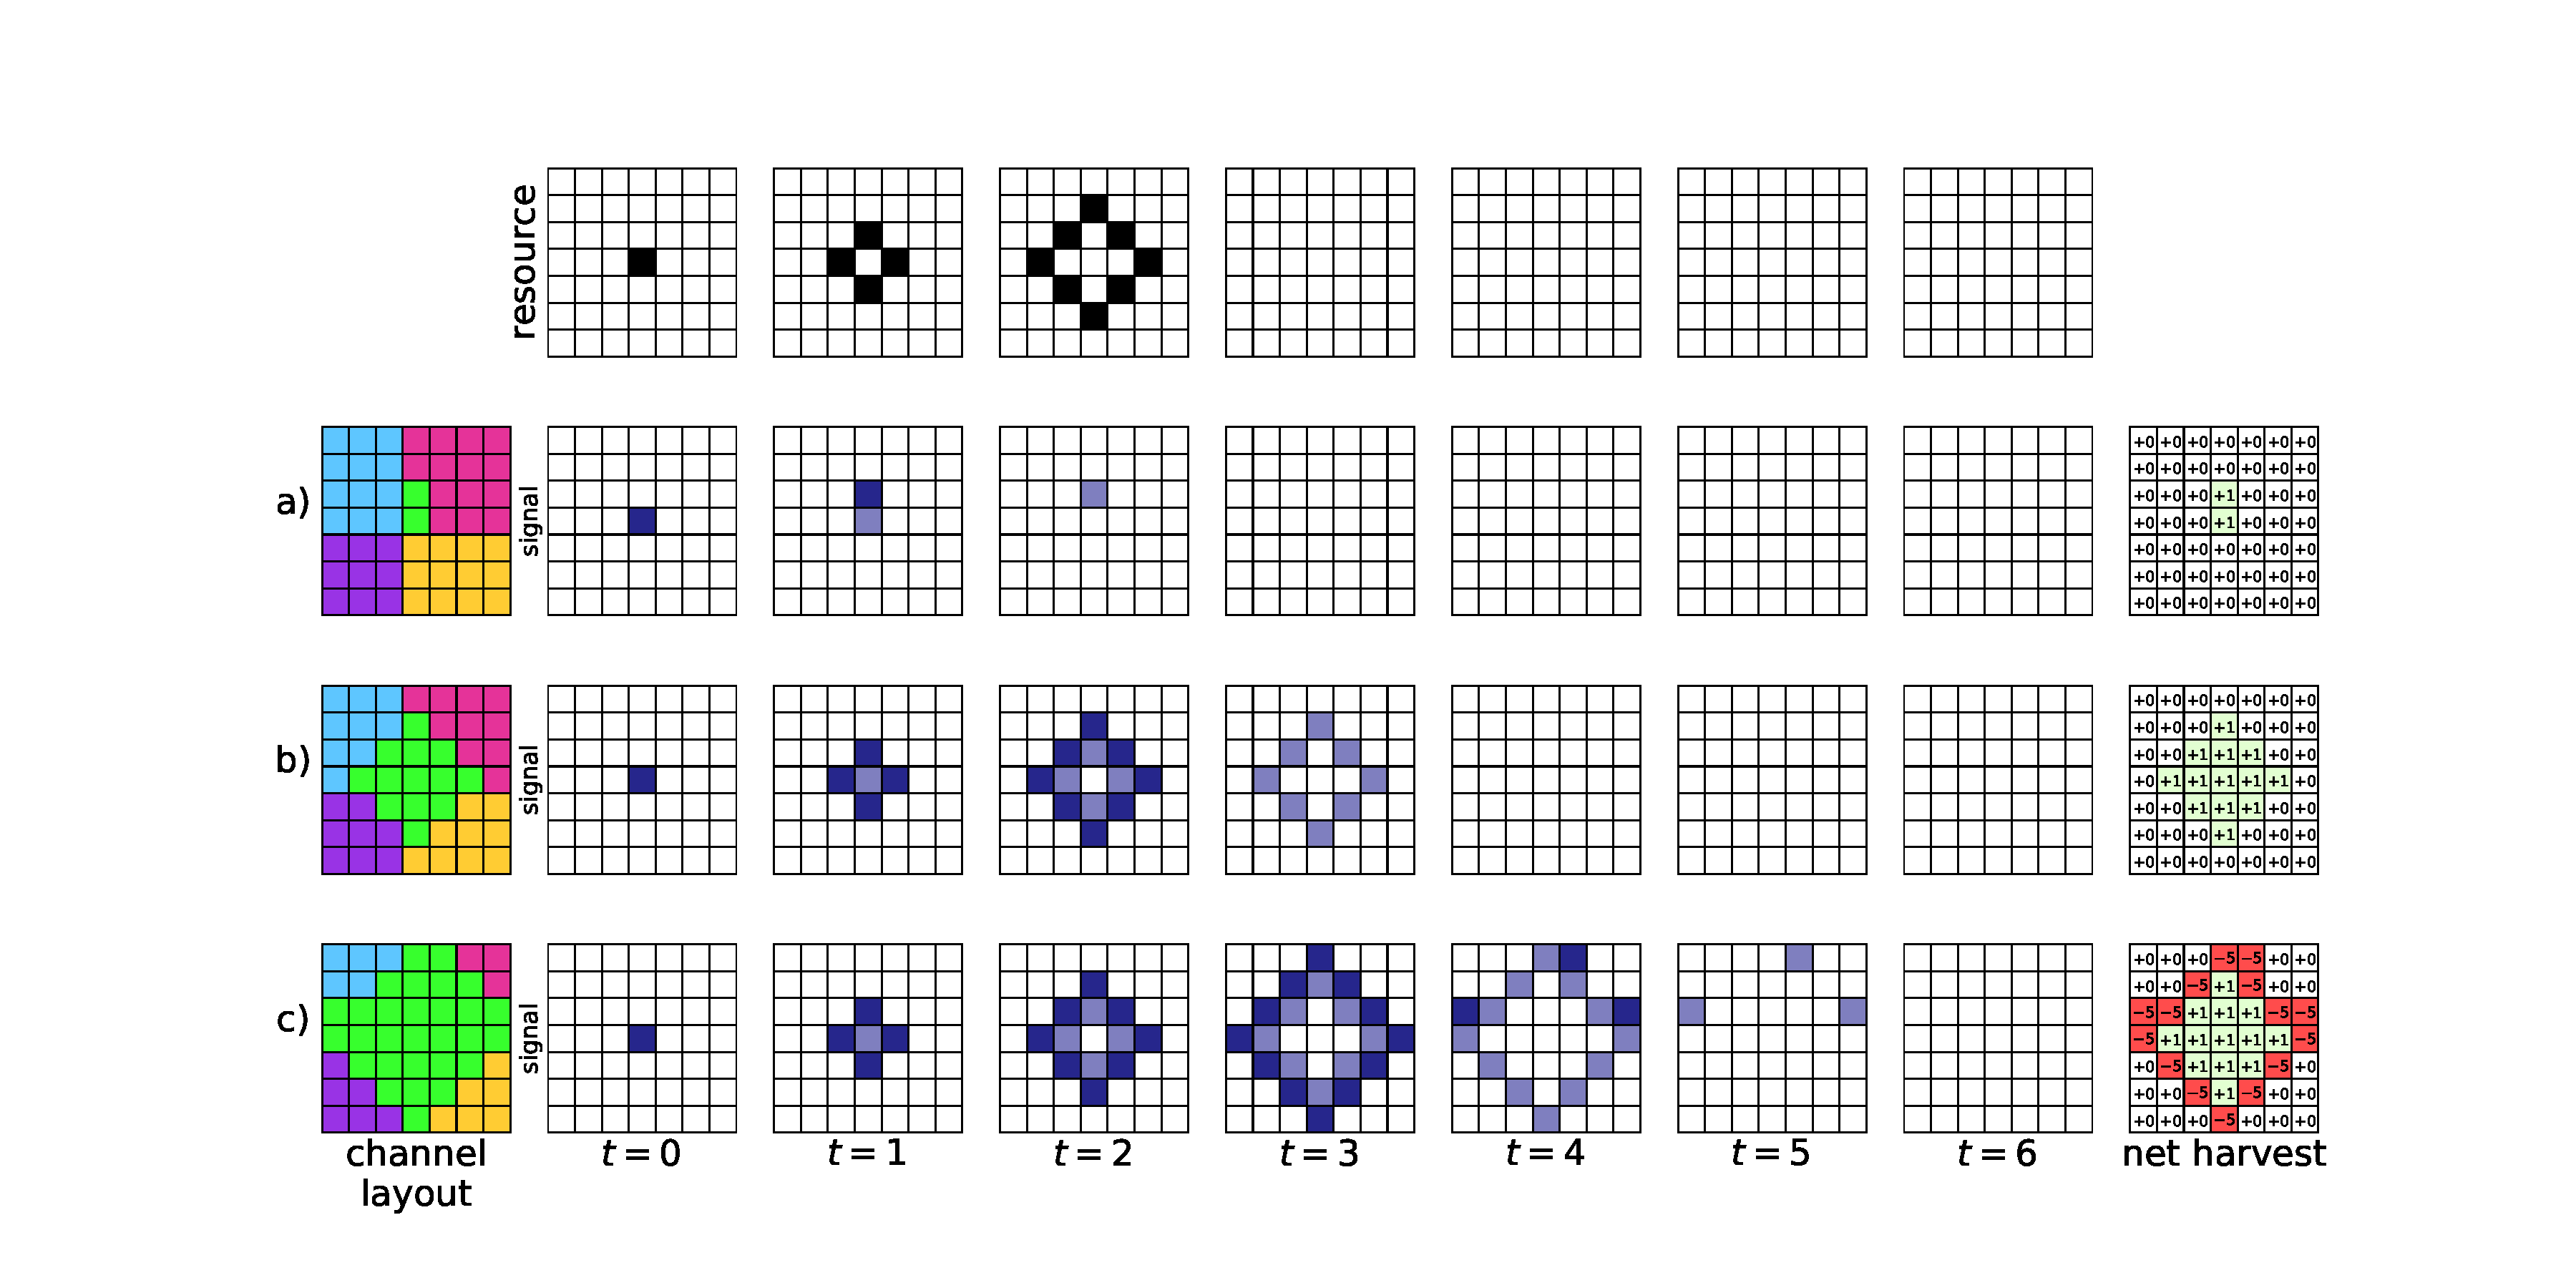
\includegraphics[width=2.0\columnwidth]{img/explanatory}
\caption{
\textbf{Activation signaling, and net resource collection for three different channel configurations during a resource wave event.}
At the top, a resource wave is depicted propagating over three updates and then ceasing for four updates (left to right).
In row $a$, a small channel-signaling group (far left, in green) is activated; tracking the resource wave (top) yields a small net resource harvest (far right).
In row $b$, an intermediate-sized channel-signaling group yields a high net resource harvest.
Finally, in row $c$, a large channel-signaling group incurs a net negative resource harvest.
In rows $a$, $b$, and $c$, dark purple indicates the active state, light purple indicates the quiescent state, and white indicates the ready state.
}
\label{fig:explanatory}
\end{center}
\end{figure*}


We will begin by discussing the implementation of our artificial environment at a single hierarchicical level, then lay out how the system scales to multiple levels.
As shown Figure \ref{fig:explanatory}, resource is distributed in waves that emanate from a single point.
With each simulation update, the resource wave advances one grid tile outward until it reaches a predefined extent.
The resource wave then ceases.
Coincident with the inception of each resource wave, an activation-quiescence signal wave is triggered at the wave's center point.
Example signal waves are shown in Figure \ref{fig:explanatory}.
With every update, the signal wave passes to adjoining cells registered to the same channel as the cell it emanates from.
The signal wave is not propagated to any cells on any other channel.
In this way, cells sharing the channel of the cell where the resource wave originated are activated coincident with the resource wave.

In order to obtain resource, a cell must be activated by a signal wave as the resource wave passes over.
The cell at the center of a resource wave will always be activated and absorb resource.
However, immediately adjacent cells can only obtain resource by the action of the signal wave --- by sharing the channel of the originating cell.
Cells further off depend on a continuous path of cells extending from the originating cell that signal on the originating channel in order to obtain resource.
As shown in Example $a$ of Figure \ref{fig:explanatory}, the rate of resource collection is determined by the size of a channel signaling network; small or fragmented channel networks will tend to frequently miss out on resource as it passes over.

Importantly, a significant activation cost is paid by each cell that is activated by a signal wave.
This activation cost is outweighed by the amount of resource collected --- cells that activate in concert with a resource wave take away a net benefit.
Recall, though, that resource waves have a limited extent.
Cells that activate outside of the extent of the resource wave or activate out of sync with the resource wave (i.e. are not connected via a direct path to the originating cell) pay a cost.
Cells that frequently activate erroneously go bankrupt and die.
This scenario is depicted in Example $c$ of Figure \ref{fig:explanatory}.

In this manner, ``Goldilocks'' --- not to small and not too big --- same-channel signaling networks are selected for.
In our implementation, resource waves are seeded at a single location drawn  with uniform probability from the toroidal grid.
Based on this location, resource wave seeds are tiled over the toroidal grid so as to have kissing --- but not overlapping --- extents.
All the waves are updated to completion in synchrony.
Then, another batch of resource waves is seeded.
This process ensures that selection for ``Goldilocks'' same-channel signaling networks is uniformly distributed over the toroidal grid.

When organisms accrue sufficient resources, they may choose to pay a cost reproduce.
Organisms may control the size and shape of their same-channel signaling group by strategic control of reproduction.
Three choices are afforded: whether to reproduce at all, where among the four adjoining tiles of the toroidal grid to place their offspring, and whether the offspring should be registered to the parent's signaling channel or should instead be registered to a randomly chosen signaling channel.

hierarchy

channels are nested -- like provinces in a country.
Each country is subdivided into provinces.
No province is in two countries!

\subsection{test organisms}

each organism consisted of a set of 15 floating-point values clamped to the range $[0,1]$ that described the following set of stochastic strategies.

$P_0, P_1, P_2$
res-pool

sorted from inside out

$A_0, A_1$
avoid-over

$E_0, E_1, E_2$
endowment

$C_0, C_1$
off-ch-cap

$S_0, S_1$
sort-off

$M_0, M_1, M_2$
damage-suicide

We would expect a zero-level individual to exhibit a genotype along the lines of

describe

We would expect a first-level individual to exhibit a genotype along the lines of

describe



We would expect a second-level individual to exhibit a genotype along the lines of

describe

\subsection{implementation}

code is available here \url{https://github.com/mmore500/dishtiny}

data and visualizations are available here \url{https://osf.io/ewvg8/}
